% vim: set tw=78 sts=2 sw=2 ts=8 aw et ai:
\documentclass{soa.cs.pub.ro}

\usepackage{code/highlight}
\usepackage{color}
\usepackage{alltt}
\usepackage{verbatim}
\usepackage{listings}
\usepackage[absolute,overlay]{textpos}

\title[Performance of Web Protocols]{Comparative Analysis of Performance Using
Server-Client Protocols}
\subtitle{Mihail Costea \& Liviu Chircu (\textit{The Penguins})}
\date{15 Jauary 2013}

\begin{document}

% Slide 1
\frame{\titlepage}

% Slide 2
\frame{\tableofcontents}

% Slide 3
\section{First half (recap)}

% Slide 4
\begin{frame}{Initial Research: Related Work}
  \begin{itemize}
    \item WebSocket-based clients require:
      \begin{itemize}
        \item constant memory (AJAX-based: increasing rates!) [3]
        \item 50\% less network bandwith [3]
      \end{itemize}
    \item for 2B of data per frame exchanged by WebSockets, AJAX enchanges
      up to 8KB of HTTP headers [4]
  \end{itemize}
\end{frame}

% Slide 5
\begin{frame}{Initial Performance Evaluation Framework}
  \begin{figure}
     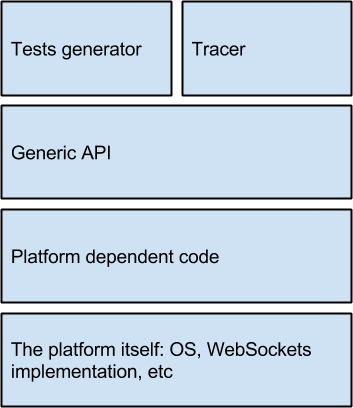
\includegraphics[scale=0.32]{img/architecture.png}
  \end{figure}
  \begin{itemize}
    \item Advantages:
      \begin{itemize}
        \item profiling flexibility
        \item platform independent
      \end{itemize}
  \end{itemize}
\end{frame}

% Slide 6
\section{The "Tests Generator"}

% Slide 7
\begin{frame}{The "Tests Generator"}
  \begin{itemize}
    \item Architectural goals:
      \begin{itemize}
        \item several WebSocket clients
        \item all kinds of stress testing scenarios
        \item assess CPU, RAM and network throughput
      \end{itemize}
    \item Final implementation:
      \begin{itemize}
        \item \textbf{ws} and \textbf{WebSocket-Node} as clients (from Node.js)
        \item obtain CPU and Memory Consumption using the \textbf{Look}
              profiler for Node.js apps [5]
      \end{itemize}
  \end{itemize}
\end{frame}

% Slide 8
\begin{frame}{The "Tests Generator"}
  \begin{itemize}
    \item Testing scenarios included:
      \begin{itemize}
        \item 4 new clients/second, minimal data
        \item 600 new clients/120 seconds, minimal data
        \item 100 clients, exchanging data starting at 2KB, up to 1MB (+2KB/s)
        \item 400 clients, minimal data, close connection,
              add 200 clients. repeat
      \end{itemize}
  \end{itemize}
\end{frame}

% Slide 9
\begin{frame}{Putting the "Tests Generator" to work}
  \begin{columns}
    \begin{column}[l]{0.45\textwidth}
      \begin{center}
        Testing Scenario 1
      \end{center}
      \begin{figure}
         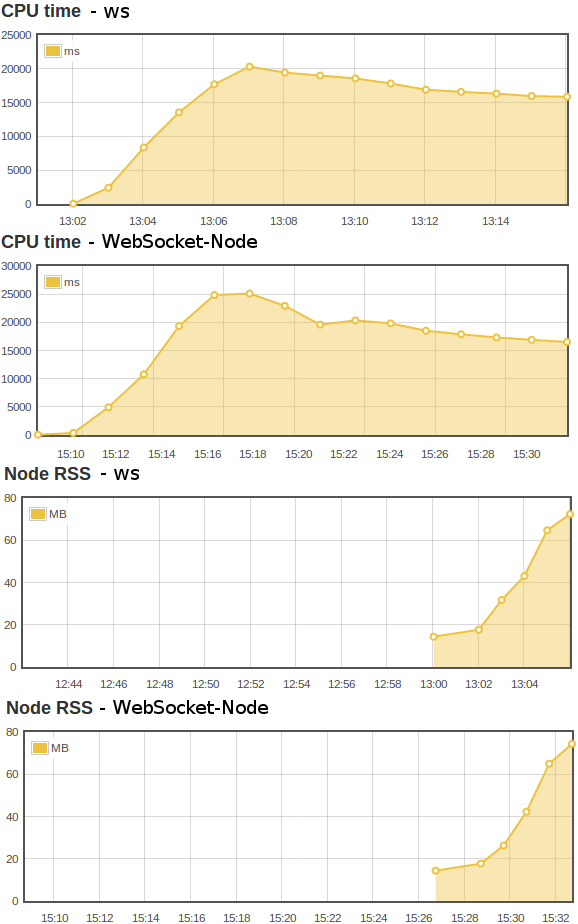
\includegraphics[scale=0.18]{img/test1v2.png}
      \end{figure}
    \end{column}
    \begin{column}[l]{0.45\textwidth}
      \begin{center}
        Testing Scenario 3
      \end{center}
      \begin{figure}
         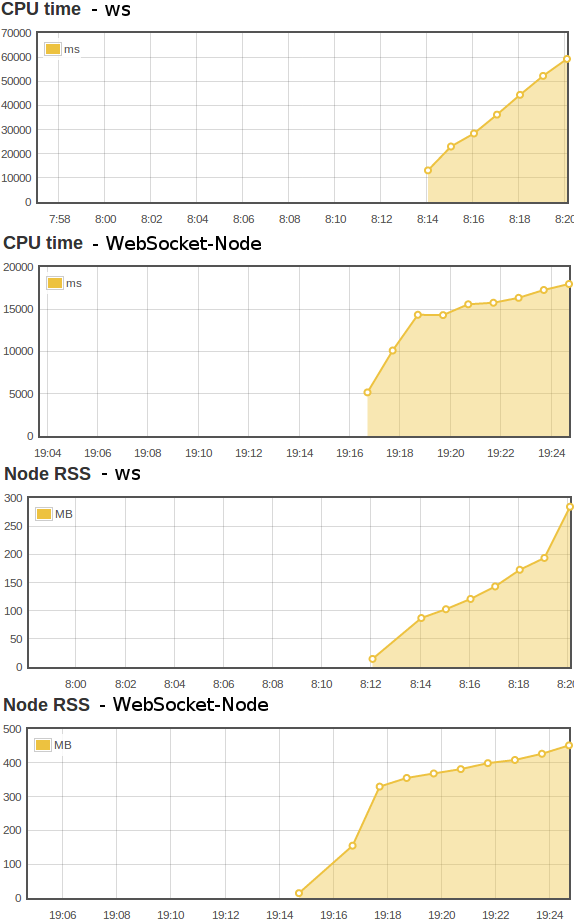
\includegraphics[scale=0.18]{img/test3v2.png}
      \end{figure}
    \end{column}
  \end{columns}
\end{frame}

% Slide 10
\section{Updated Architecture Proposal}

% Slide 11
\begin{frame}{The Alternate Design}
  \begin{itemize}
    \item Core ideas:
      \begin{itemize}
        \item learning and also using a new API can be painful
        \item users would preffer a "black-box" evaluation framework
      \end{itemize}
    \item An alternate design:
      \begin{figure}
         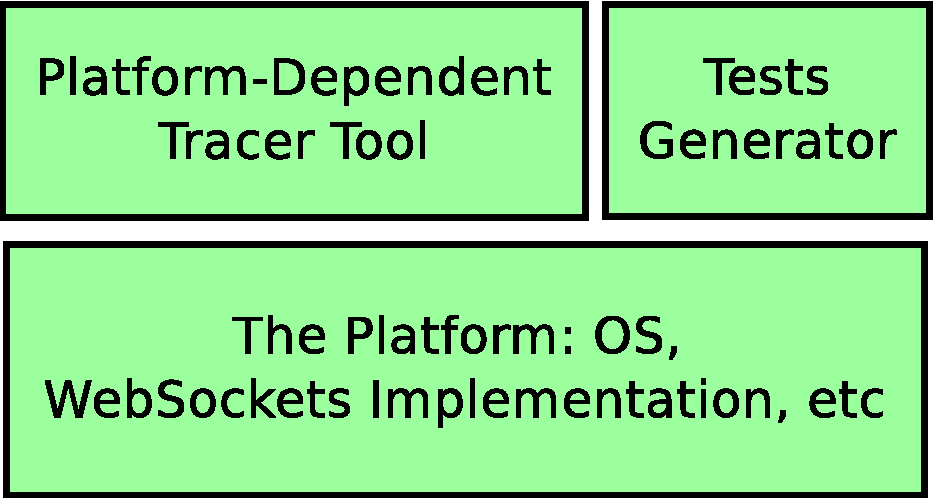
\includegraphics[scale=0.25]{img/architecture2.pdf}
      \end{figure}
  \end{itemize}
\end{frame}

\begin{frame}{Other resources}
  \begin{itemize}
    \item [1] Anthony T. Holdener, III. Ajax: The Definitive Guide
    \item [2] A. Melnikov I. Fette. The websocket protocol, 2011
    \item [3] D.G. Puranik, D.C. Feiock, and J.H. Hill. Real-time
              monitoring using ajax and websockets.
    \item [4] Ian Hickson.
      http://www.ietf.org/mail-archive/web/hybi/current/msg00784.html
    \item [5] S. Agarwal. Real-time web application roadblock: Performance
      penalty of html sockets.
  \end{itemize}
\end{frame}

\section{Questions}

\end{document}
